\subsection{Sensitivity analysis and numerical experiments}
\label{sec:q1e}

We vary the tariff discount $\beta^{\mathrm{DSO}}$, cap factor $f$,
and exceedance penalty $\alpha^{\mathrm{DSO}}$ one at a time around
$(0.75,1.3,10)$. The member data and battery terminal conditions
are fixed. The reference dispatch and individual cap shares
$\kappa_i$ are computed once. The sweeps cover $\beta^{\mathrm{DSO}}\in[0,1]$,
$f\in[0.65,8]$, and $\alpha^{\mathrm{DSO}}\in[0,30]$~DKK/kWh.
Signing thresholds satisfy $J^m=J^{\mathcal R}$ and are refined by
bisection. All six base-case metrics match the preceding analysis.

\paragraph{Tariff discount.}
Figure~\ref{fig:q1-sensitivity-beta} shows that both contract costs
fall as the discount rises. The community contract breaks even
against $\mathcal R$ at
\begin{equation}
\beta_{\mathrm{crit}}^{\mathcal C}\simeq0.4838,
\qquad J^{\mathcal C}=J^{\mathcal R}\simeq398.24~\mathrm{DKK}.
\label{eq:q1-discount-threshold}
\end{equation}
Individual contracts still cost 458.05~DKK at a full discount.
The collective savings relative to individual contracts rise
from 101.70 to 110.75~DKK between the sweep endpoints.

The discount changes the objective coefficients. The Lagrangian
envelope relation gives the local cost slope as the negative of
undiscounted tariff charges on within-cap imports and exports
at the optimal dispatch. At the base point, increasing
the discount by one percentage point saves approximately
0.99~DKK in $\mathcal C$ and 0.87~DKK in $\mathcal I$.

\begin{figure}[htbp]
    \centering
    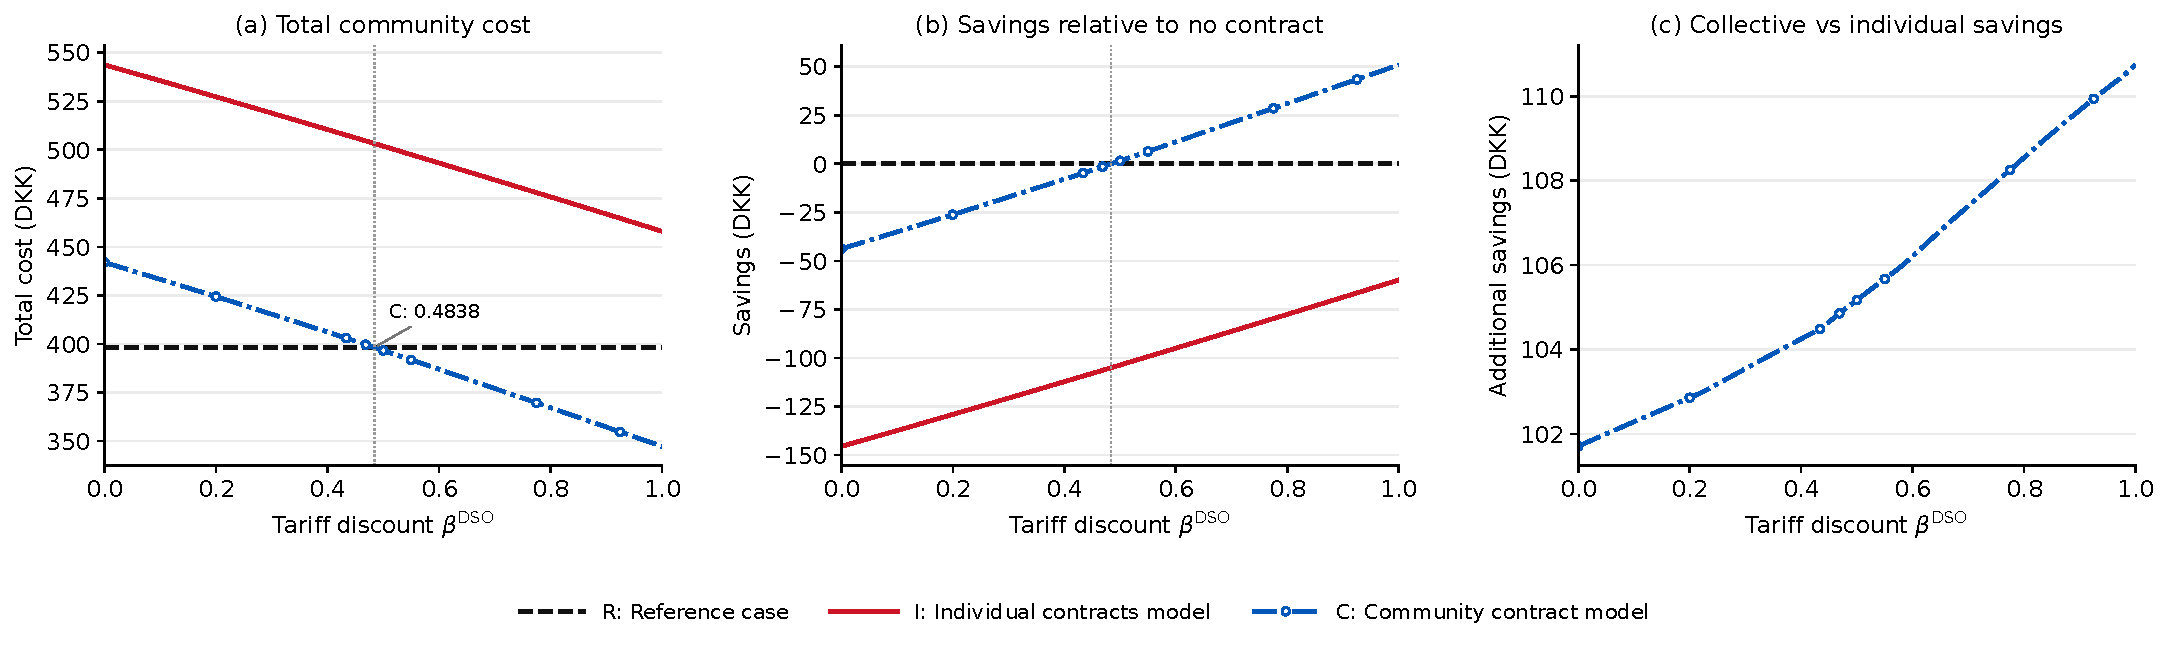
\includegraphics[width=0.99\linewidth]{results/sensitivity/sensitivity_beta.pdf}
    \caption{Total cost and savings against the tariff discount at
    $f=1.3$ and $\alpha^{\mathrm{DSO}}=10$~DKK/kWh. The dotted lines
    mark the community signing threshold.}
    \label{fig:q1-sensitivity-beta}
\end{figure}

\paragraph{Hourly import cap.}
Following Table~11, the capacity profiles are
\begin{equation}
\overline P_t^{\mathrm{DSO}}(f)
=\frac{f}{1.3}\overline P_t^{\mathrm{DSO,base}},
\qquad
\overline P_{i,t}^{\mathrm{DSO}}(f)
=\kappa_i\overline P_t^{\mathrm{DSO}}(f).
\label{eq:q1-cap-scaling}
\end{equation}
In Figure~\ref{fig:q1-sensitivity-f}, both costs fall as the cap
is relaxed. The signing thresholds are
\begin{equation}
f_{\mathrm{crit}}^{\mathcal C}\simeq1.1388,
\qquad
f_{\mathrm{crit}}^{\mathcal I}\simeq1.8475.
\label{eq:q1-cap-thresholds}
\end{equation}
Increasing $f$ from 1.3 to 2 lowers $J^{\mathcal C}$ from
372.16 to 336.65~DKK and raises its peak from 9.390 to
14.446~kW. Community exceedance is zero at both caps.
Collective savings relative to individual contracts fall from
107.97~DKK at $f=1.3$ to 21.64~DKK at $f=3$.

Away from breakpoints, the cost slope for $\mathcal C$ is
$-\sum_t\chi_t^{\mathcal C}\overline P_t^{\mathrm{DSO,base}}/1.3$,
where $\chi_t^{\mathcal C}$ is the cap multiplier. For
$\mathcal I$, the corresponding sum uses the individual
multipliers and weights each cap increment by $\kappa_i$.
At $f=1.3$, the selected cap multipliers give cost slopes of
$-192.81$ for $\mathcal I$ and $-125.97$ for $\mathcal C$ in DKK
per unit of $f$. The individual caps therefore have a higher
marginal value at the base case. At $f=2$, the community slope
falls in magnitude to 24.28~DKK per unit of $f$.

\begin{figure}[htbp]
    \centering
    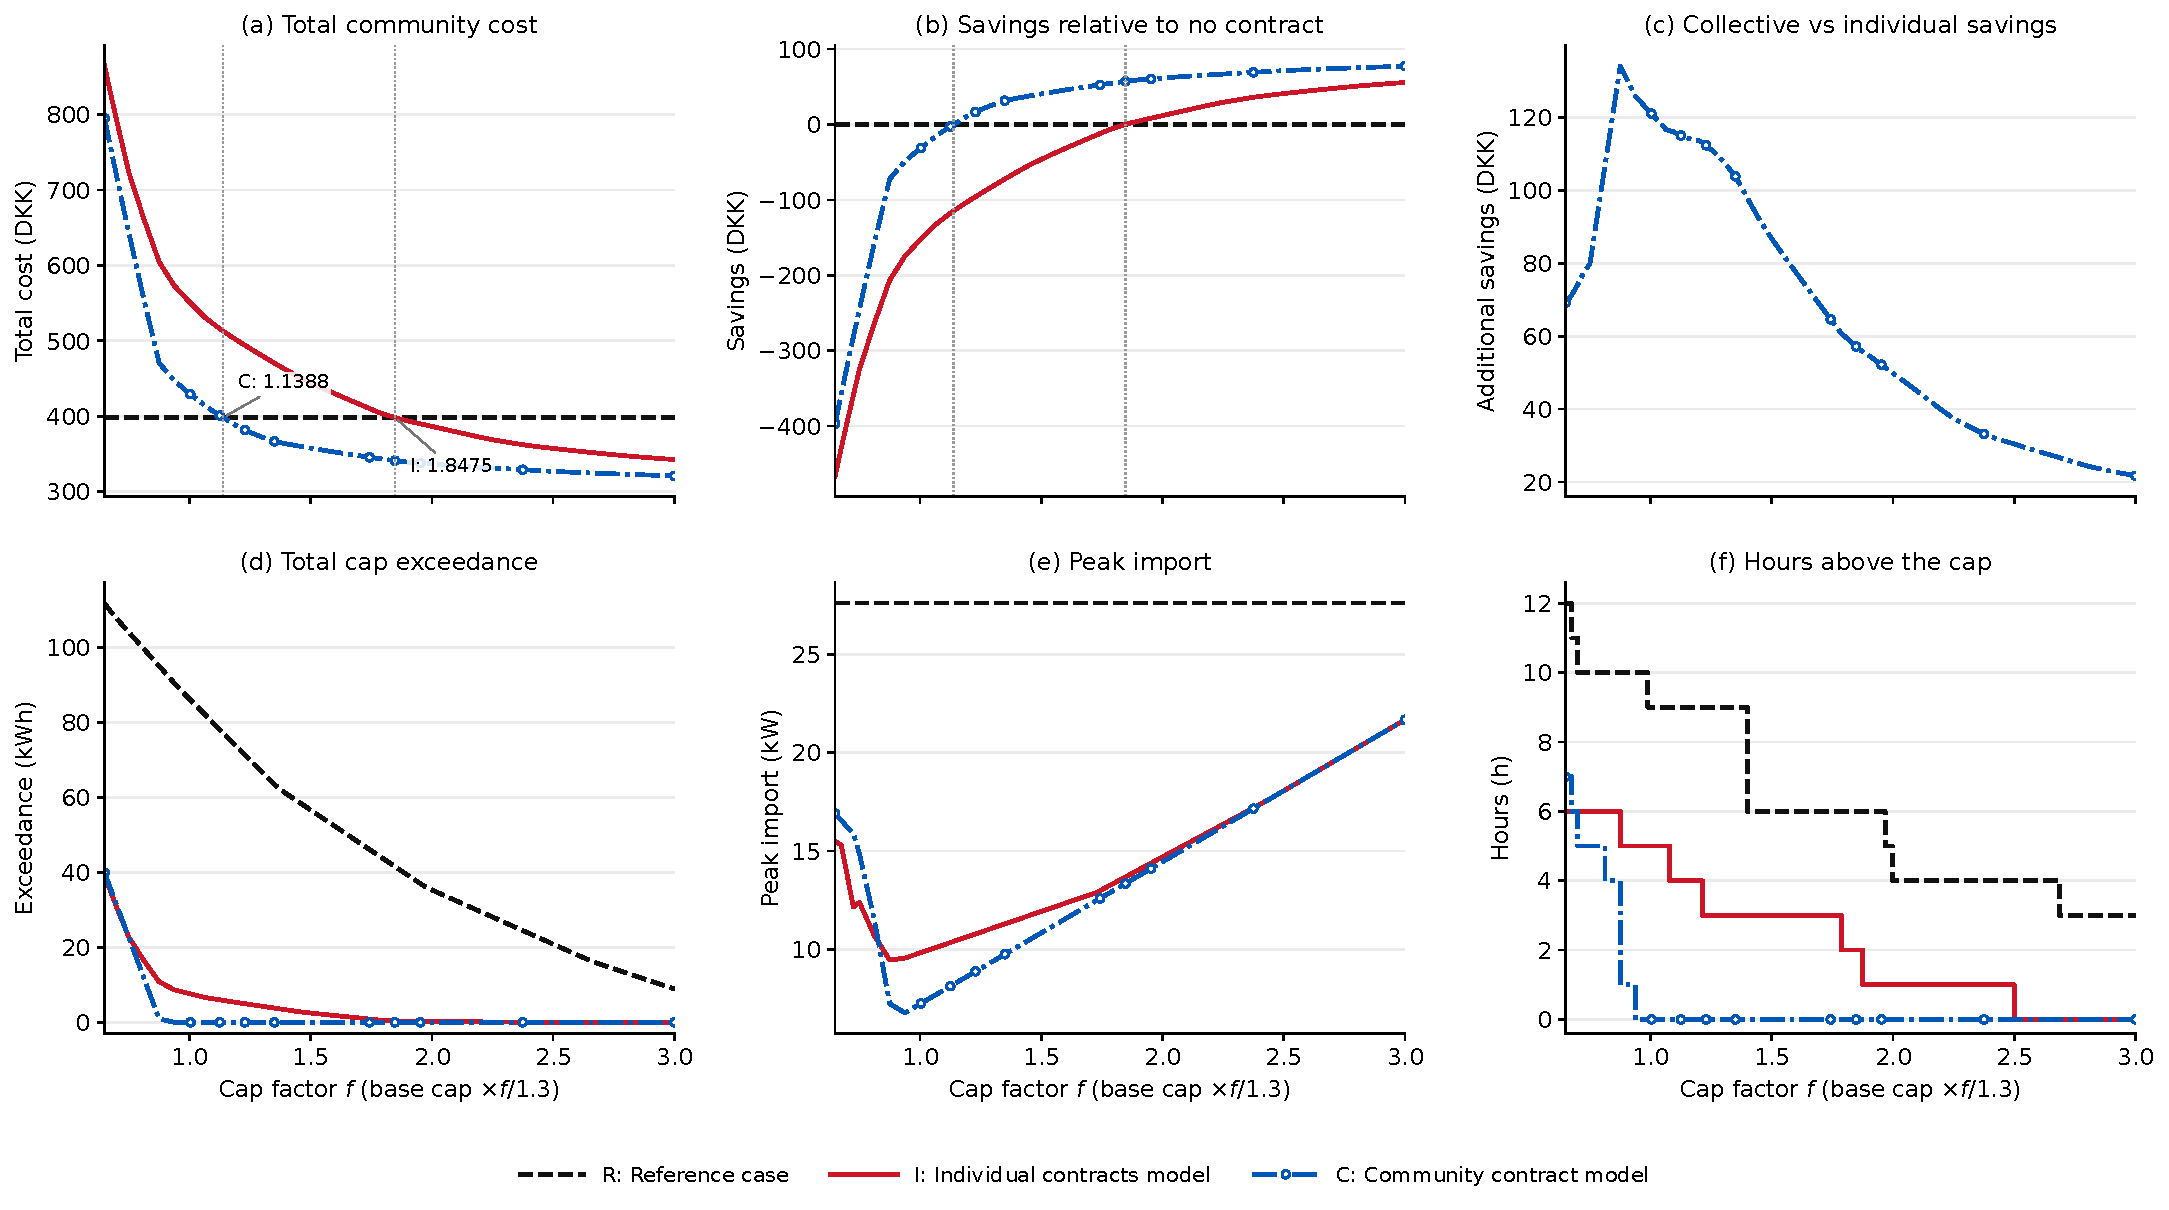
\includegraphics[width=0.99\linewidth]{results/sensitivity/sensitivity_f.pdf}
    \caption{Six contract-value metrics against the cap factor
    at $\beta^{\mathrm{DSO}}=0.75$ and
    $\alpha^{\mathrm{DSO}}=10$~DKK/kWh. The displayed range
    is $f\in[0.65,3]$.}
    \label{fig:q1-sensitivity-f}
\end{figure}

\paragraph{Exceedance penalty.}
The full penalty sweep shows that raising the penalty from 0.5 to
10~DKK/kWh cuts feeder exceedance from 65.005 to
4.288~kWh in $\mathcal I$ and from 54.926 to zero in $\mathcal C$.
Figure~\ref{fig:q1-sensitivity-alpha} shows the low-penalty range.
The hours above the cap fall from eight to three and from five to zero,
respectively, between the two full-sweep points. Individual contracts
become more expensive than $\mathcal R$ above
\begin{equation}
\alpha_{\mathrm{crit}}^{\mathcal I}\simeq1.4954~\mathrm{DKK/kWh}.
\label{eq:q1-penalty-threshold}
\end{equation}
The community contract remains cheaper than $\mathcal R$ throughout
the sweep. Its cost levels off at 372.16~DKK once exceedance
reaches zero at about 4.310~DKK/kWh. Individual contracts reach
their minimum charged exceedance of 4.288~kWh at about
5.066~DKK/kWh.

The community balance multiplier satisfies
$\lambda_t^{\mathcal C}\le p_t+\alpha^{\mathrm{DSO}}$, with equality
when $x_t>0$. Thus, the penalty raises the marginal cost of importing
above the cap. Away from breakpoints, the cost slope with respect to the penalty equals
total charged exceedance. Above the respective thresholds, the slope is zero in $\mathcal C$
and 4.288 in $\mathcal I$. Raising the penalty from
10 to 20~DKK/kWh adds 42.88~DKK to $J^{\mathcal I}$.

\begin{figure}[htbp]
    \centering
    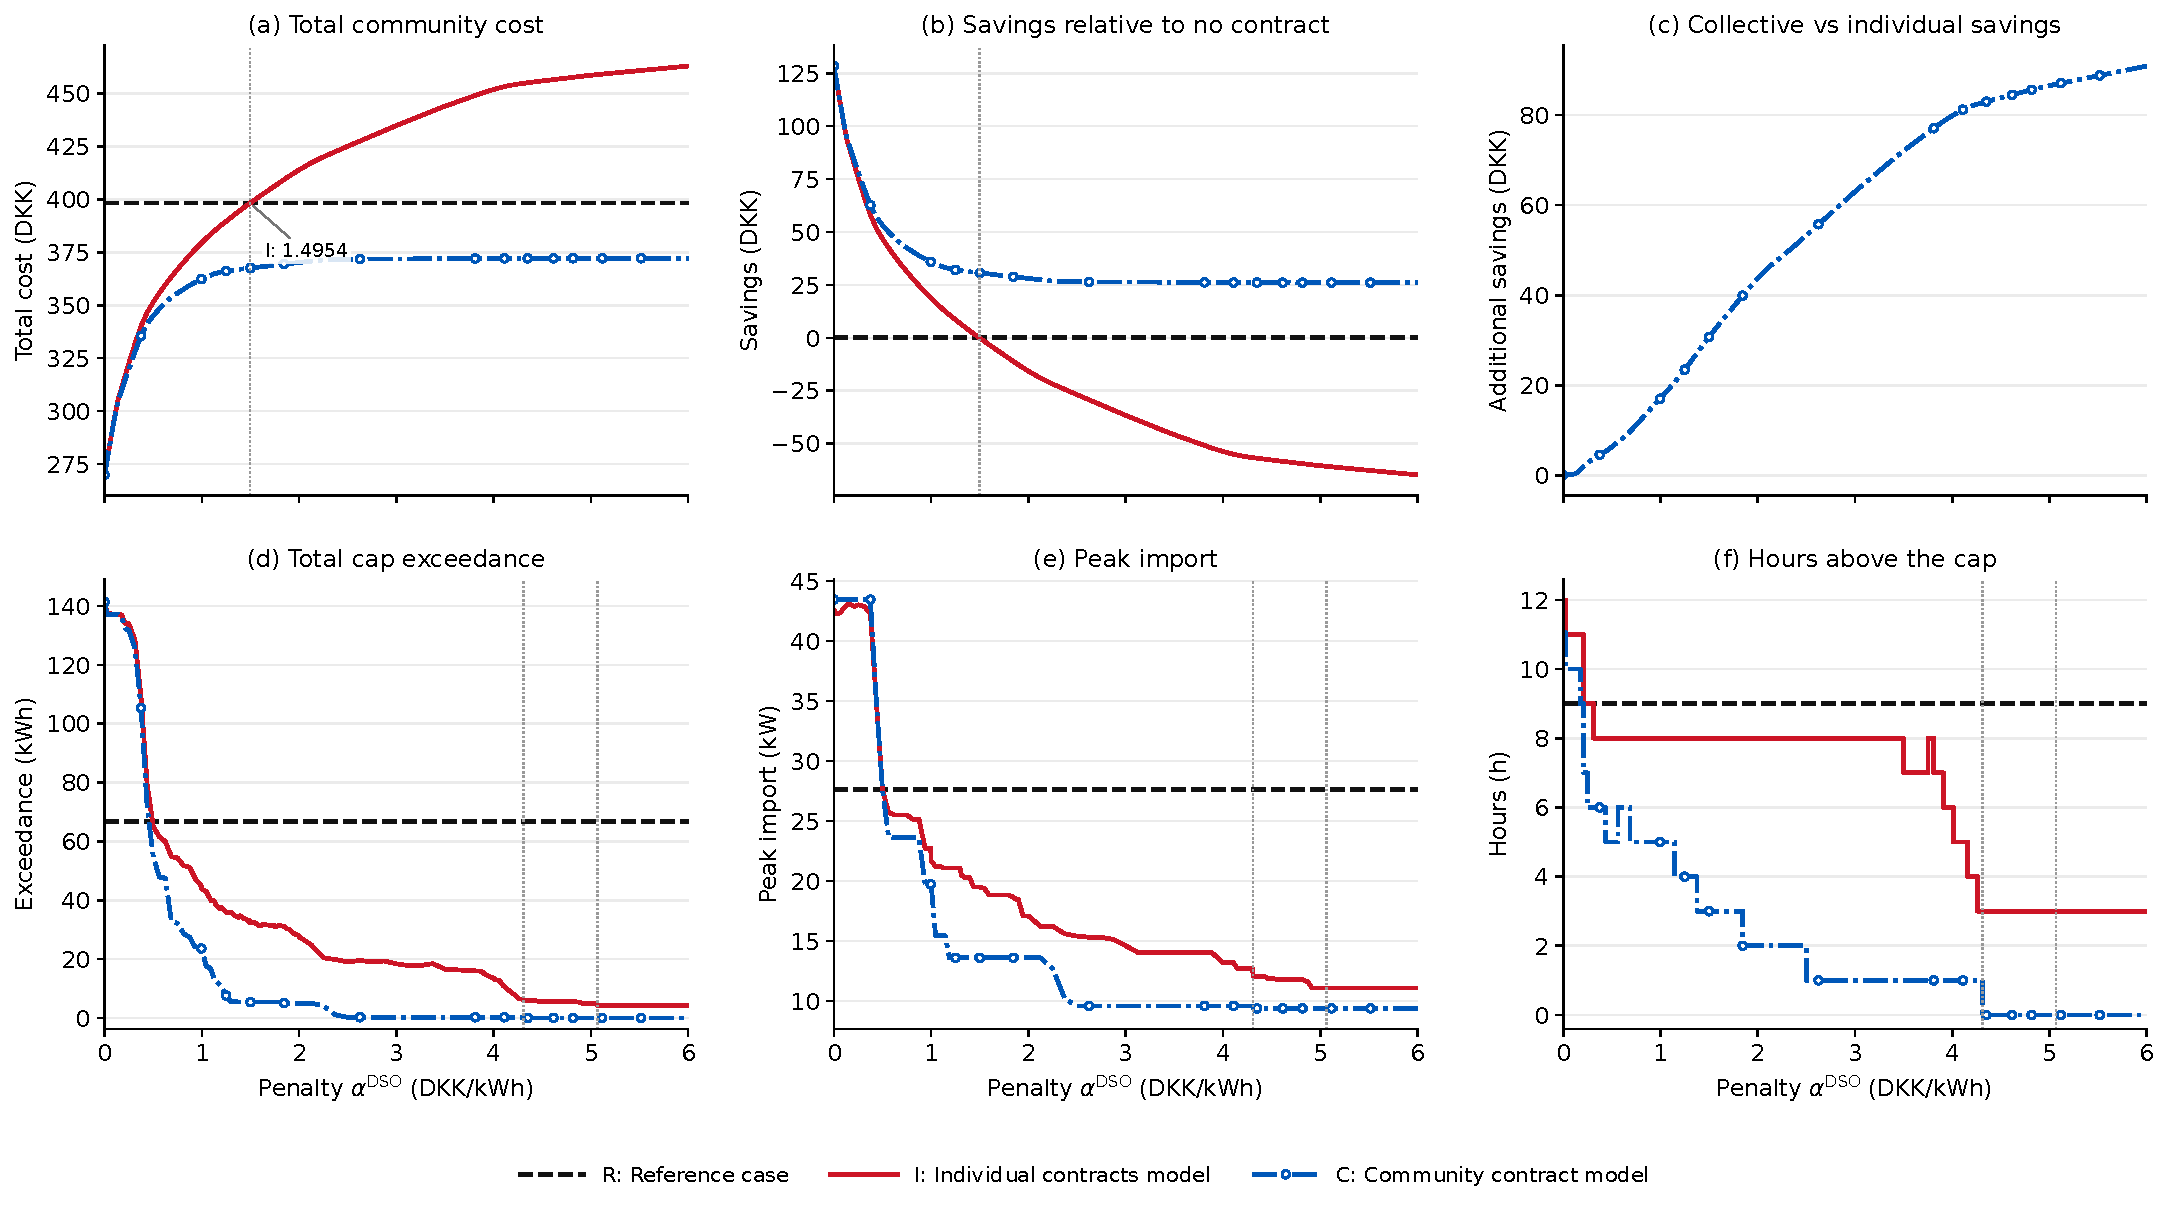
\includegraphics[width=0.99\linewidth]{results/sensitivity/sensitivity_alpha.pdf}
    \caption{Six contract-value metrics against the exceedance penalty
    at $\beta^{\mathrm{DSO}}=0.75$ and $f=1.3$. The displayed range
    is $[0,6]$~DKK/kWh.}
    \label{fig:q1-sensitivity-alpha}
\end{figure}
